\documentclass[12pt]{article}
\usepackage[utf8]{inputenc}
\usepackage{graphicx}
\usepackage{float}
\usepackage{amsmath}
\usepackage{booktabs}
\usepackage{geometry}
\geometry{margin=1in}

\title{Assignment 4 – Machine Learning \\ \large Questions 1 to 3}
\author{Group 15}
\date{}

\begin{document}

\maketitle

\section*{Introduction}

The objective of this assignment is to develop and evaluate tree-based models for predicting whether a subject with Mild Cognitive Impairment (MCI) will convert to Alzheimer’s Disease (progressive MCI or pMCI) or remain stable (stable MCI or sMCI) based on glucose metabolism features from 14 cortical brain regions.

\section*{Question 1 – Decision Tree Classifier}

We trained a \textbf{Decision Tree Classifier} using a grid search to optimize the \texttt{criterion} hyperparameter among \texttt{gini}, \texttt{entropy}, and \texttt{log\_loss}. The dataset included 202 sMCI and 202 pMCI individuals for training, and 361 sMCI and 194 pMCI individuals for testing.

\subsection*{Best Criterion}
The best performing criterion found was \texttt{gini}.

\subsection*{Performance on Test Data}
\begin{itemize}
    \item Accuracy: 59.1\%
    \item Precision: 44.5\%
    \item Recall (Sensitivity): 69.1\%
    \item Specificity: 53.7\%
    \item Balanced Accuracy: \textbf{61.4\%}
\end{itemize}

\subsection*{Discussion}
The decision tree shows reasonable recall for the pMCI class, but suffers from relatively low specificity and precision. The model likely overfits due to its complexity and limited generalization capacity, as reflected by the moderate balanced accuracy.

\subsection*{Tree Visualization}
Figure~\ref{fig:tree} displays the structure of the trained Decision Tree.

\begin{figure}[H]
    \centering
    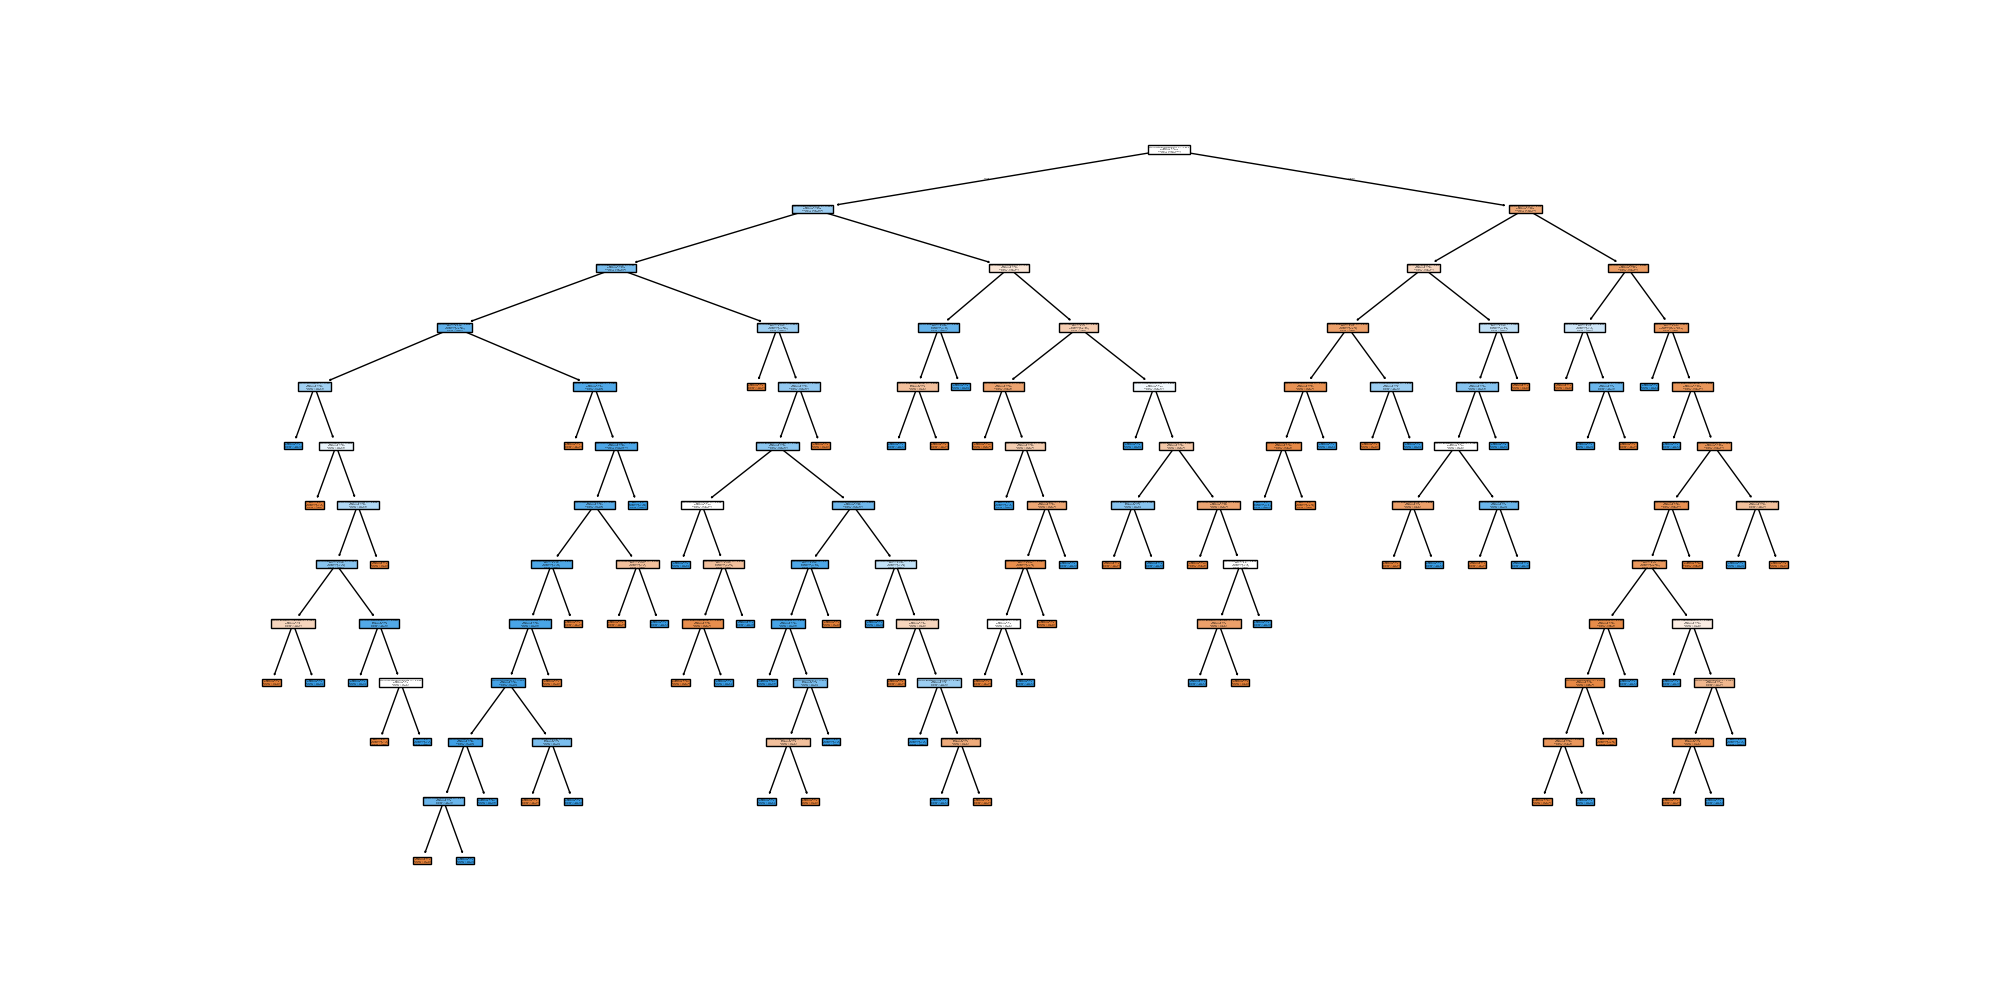
\includegraphics[width=\textwidth]{IMG/Figure_1.png}
    \caption{Trained Decision Tree Classifier}
    \label{fig:tree}
\end{figure}

\section*{Question 2 – Analysis of the Tree Structure}

The Decision Tree uses multiple features repeatedly, particularly in early splits, indicating higher importance. From visual inspection of the tree, the most frequently used features near the root include:

\begin{itemize}
    \item \texttt{ctx-rh-precuneus}
    \item \texttt{ctx-lh-inferiorparietal}
    \item \texttt{ctx-lh-middletemporal}
\end{itemize}

This suggests these regions may carry stronger predictive signals for distinguishing sMCI and pMCI classes in this dataset.

\section*{Question 3 – Random Forest Classifier}

We trained a \textbf{Random Forest Classifier} using GridSearchCV to tune the number of estimators (\texttt{n\_estimators} = 100 or 200) and the splitting criterion (\texttt{gini}, \texttt{entropy}, or \texttt{log\_loss}).

\subsection*{Best Parameters}
\begin{itemize}
    \item \texttt{criterion}: \texttt{entropy}
    \item \texttt{n\_estimators}: 100
\end{itemize}

\subsection*{Performance on Test Data}
\begin{itemize}
    \item Accuracy: 64.5\%
    \item Precision: 49.5\%
    \item Recall (Sensitivity): 78.4\%
    \item Specificity: 57.1\%
    \item Balanced Accuracy: \textbf{67.7\%}
\end{itemize}

\subsection*{Discussion}
The Random Forest model significantly outperforms the single Decision Tree in terms of recall and balanced accuracy. This reflects the advantage of ensembling in reducing overfitting and increasing generalization.

Additionally, feature importance analysis highlights several regions consistently contributing to the classification, though the predictive signal remains weak overall, likely due to the subtle nature of pMCI conversion patterns.

\section{Question 4}

After extensive hyperparameter tuning using grid search with cross-validation on a Random Forest classifier, the best model was selected based on balanced accuracy. The final chosen model uses the \texttt{entropy} criterion, \texttt{class\_weight="balanced"}, \texttt{n\_estimators=200}, \texttt{max\_depth=20}, and \texttt{min\_samples\_split=5}. This configuration achieved the highest validation balanced accuracy of 66.98\%.

However, this performance remains considerably lower than what was observed in previous assignments using SVM-based approaches. Despite optimization efforts, tree-based classifiers do not appear to generalize well on this dataset. This suggests that the underlying decision boundaries may not be well captured by tree-based models, and alternative approaches such as kernel methods might be better suited for this classification task.

\end{document}
